\documentclass{standalone}
\usepackage{tikz}
\usepackage{animate}
\usepackage{amsmath}
\usepackage{ifthen}
\usetikzlibrary {matrix}
\usepackage{tikzlings}
\usepackage{tikzlings-penguins}

\begin{document}
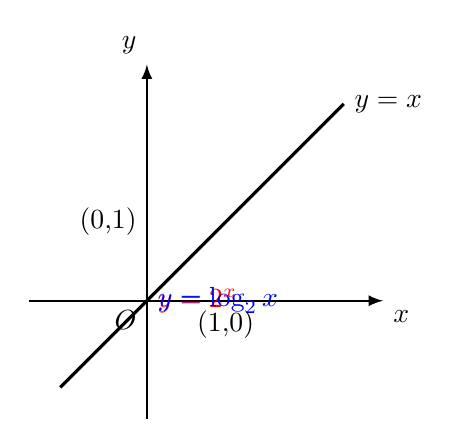
\begin{tikzpicture}[>=latex,  thick]
  \begin{scope}
    \draw[->] (-1.5,0) --(3,0) node[below right] {$x$};
    \draw[->] (0,-1.5) --(0,3) node[above left]  {$y$};
    \draw[domain=-1.1:2.5,very thick] plot (\x,\x) node[right] {$y=x$};
    \draw[domain=-1.0:1,smooth,samples=200,red,very thick] plot[id=exp2] function { exp(x)} node[right] {$y=2^x$};
    \draw[domain=0.3:3,smooth,samples=200,blue,very thick] plot[id=log2] function { log(x)} node[right] {$y=\log_{2}{x}$};
    \node[below left]  (o) at (0,0) {$O$};
    \node[below] (x1) at (1,0) {(1,0)};
    \node[left] (y1) at (0,1) {(0,1)};
  \end{scope}

\end{tikzpicture}


\end{document}
